\chapter{Trigonometry}
Trigonometry relates angles and lengths of triangles. Figure \ref{fig:triangle} shows a right-angled triangle and conventions to label its corners, sides, and angles. In the following, we assume all triangles to have at least one right angle (90 degrees or $\frac{\pi}{2})$ as all planar triangles can be dissected into two right-angled triangles. 

\begin{figure}[!htb]
\centering
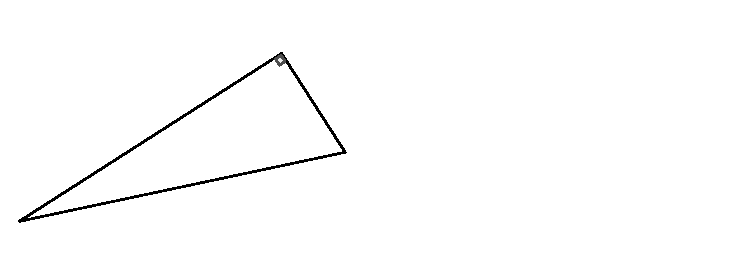
\includegraphics[width=0.8\textwidth]{figs/triangle}
\caption{Left: A right-angled triangle with common notation. Right: Trigonometric relationships on the unit circle and angles corresponding to the four quadrants. \label{fig:triangle}}
\end{figure}

The sum of all angles in any triangle is 180 degrees or $2\pi$, or 
\begin{equation}
\alpha + \beta + \gamma = 180^o
\end{equation}
If the triangle is right-angled, the relationship between edges $a$, $b$, and $c$, where $c$ is the edge opposite of the right angle is
\begin{equation}
a^2+b^2=c^2
\end{equation} 
The relationship between angles and edge lengths are captured by the trigonometric functions:
\begin{eqnarray}
\sin{\alpha}&=\frac{opposite}{hypothenuse}=\frac{a}{c}\\
\cos{\alpha}&=\frac{adjacent}{hypothenuse}=\frac{b}{c}\\
\tan{\alpha}&=\frac{opposite}{adjacent}=\frac{\sin{\alpha}}{\cos{\alpha}}=\frac{a}{b}
\end{eqnarray} 

Here, the \emph{hypothenuse}\index{Hypothenuse} is the side of the triangle that is opposite to the right angle. The \emph{adjacent} and \emph{opposite} are relative to a specific angle. For example, in Figure \ref{fig:triangle}, the adjacent of angle $\alpha$ is side $b$ and the opposite of $\alpha$ is edge $a$. 

Relations between a single angle and the edge lengths are captured by the \emph{law of cosines}\index{Law of Cosines}:
\begin{equation}
a^2=b^2+c^2-2bc\cos{\alpha}
\end{equation}

\section{Inverse trigonometry}
In order to calculate an angle given two edges, one uses inverse functions $\sin^{-1}$, $\cos^{-1}$, and $\tan^{-1}$. (Not to be confused with $\frac{1}{\sin}$ etc.) As functions can, by definition, only map one value to exactly one other value, $\sin^{-1}$ and $\tan^{-1}$ are only defined in the interval $[-90^o;+90^o]$ and $\cos^{-1}$ is defined in the interval $[0^o;180^o]$. This makes it impossible to calculate angles in the 2nd and 3rd, or the 3rd and 4th quadrant, respectively (Figure \ref{fig:triangle}). 
In order to overcome this problem, most programming languages implement a function \texttt{atan2(opposite,adjacent)}, which evaluates the sign of the numerator and denumerator, provided as two separate parameters. 

\section{Trigonometric identities}
Sine and cosine are periodic, leading to the following identities:
\begin{eqnarray}
\sin\theta=-\sin(-\theta)=-\cos(\theta+\frac{\pi}{2})=\cos(\theta-\frac{\pi}{2})\\
\cos\theta=\cos(-\theta)=\sin(\theta+\frac{\pi}{2})=-\sin(\theta-\frac{\pi}{2})
\end{eqnarray}

The sine or cosine for sums or differences between angles can be calculated using the following identities:

\begin{eqnarray}
\cos(\theta_1+\theta_2)=\cos(\theta_1)\cos(\theta_2)-\sin(\theta_1)\sin(\theta_2)\\
\sin(\theta_1+\theta_2)=\sin(\theta_1)\cos(\theta_2)+\cos(\theta_1)\sin(\theta_2)\\
\cos(\theta_1-\theta_2)=\cos(\theta_1)\cos(\theta_2)+\sin(\theta_1)\sin(\theta_2)\\
\sin(\theta_1-\theta_2)=\sin(\theta_1)\cos(\theta_2)-\cos(\theta_1)\sin(\theta_2)
\end{eqnarray}

The sum of the squares of sine and cosine for the same angle is one:
\begin{equation}
\cos(\theta)\cos(\theta)+\sin(\theta)\sin(\theta)=1
\end{equation}